\documentclass[tikz,border=6pt]{standalone}
% Shared visual language for the original benchmark atlas.
\usepackage[T1]{fontenc}
\usepackage{lmodern}
\usepackage{amsmath,amssymb}
\usetikzlibrary{arrows.meta,calc,positioning,shapes.geometric,patterns,decorations.pathmorphing,backgrounds,fit}
\definecolor{ink}{HTML}{173948}
\definecolor{flow}{HTML}{167D9A}
\definecolor{control}{HTML}{A65217}
\definecolor{measure}{HTML}{70518A}
\definecolor{pale}{HTML}{EAF2F5}
\definecolor{muted}{HTML}{526571}
\definecolor{utility}{HTML}{2E8665}
\tikzset{
  every node/.style={font=\sffamily\small,text=ink},
  equipment/.style={draw=ink,line width=1pt,fill=pale,rounded corners=2pt},
  process/.style={draw=flow,line width=1.2pt,-{Latex[length=2.5mm]}},
  signal/.style={draw=control,line width=.8pt,dashed,-{Latex[length=2mm]}},
  util/.style={draw=utility,line width=1pt,-{Latex[length=2.2mm]}},
  dimension/.style={draw=muted,line width=.6pt,{Latex[length=1.7mm]}-{Latex[length=1.7mm]}},
  labelbox/.style={fill=white,inner sep=2pt,font=\sffamily\footnotesize,align=center},
  annotation/.style={font=\sffamily\footnotesize,text=muted,align=left},
  panel/.style={draw=ink!20,fill=ink!2,rounded corners=3pt,inner sep=6pt},
  instrument/.style={circle,draw=measure,fill=white,line width=.8pt,minimum size=8mm,inner sep=1pt,font=\sffamily\scriptsize,align=center},
  port/.style={circle,fill=flow,inner sep=1.6pt},
  box/.style={equipment,minimum width=3cm,minimum height=1cm,align=center},
}
\newcommand{\atlasheader}[3]{%
  \node[anchor=north west,font=\sffamily\bfseries\LARGE] at (0,0) {#1};%
  \node[anchor=north west,font=\sffamily\small,text=muted] at (0,-.75) {Paper section #2: \textit{#3}};%
  \draw[ink!25,line width=.7pt] (0,-1.25)--(26,-1.25);%
}
\newcommand{\atlasfooter}[1]{%
  \draw[ink!25,line width=.5pt] (0,-15.8)--(26,-15.8);%
  \node[anchor=north west,annotation,text width=25.8cm] at (0,-16) {#1\\Original explanatory drawing. Source: Kroll \& Schulte (2014), DOI: 10.1016/j.asoc.2014.08.034. Model variants are identified in the accompanying case sheet.};%
}

\begin{document}
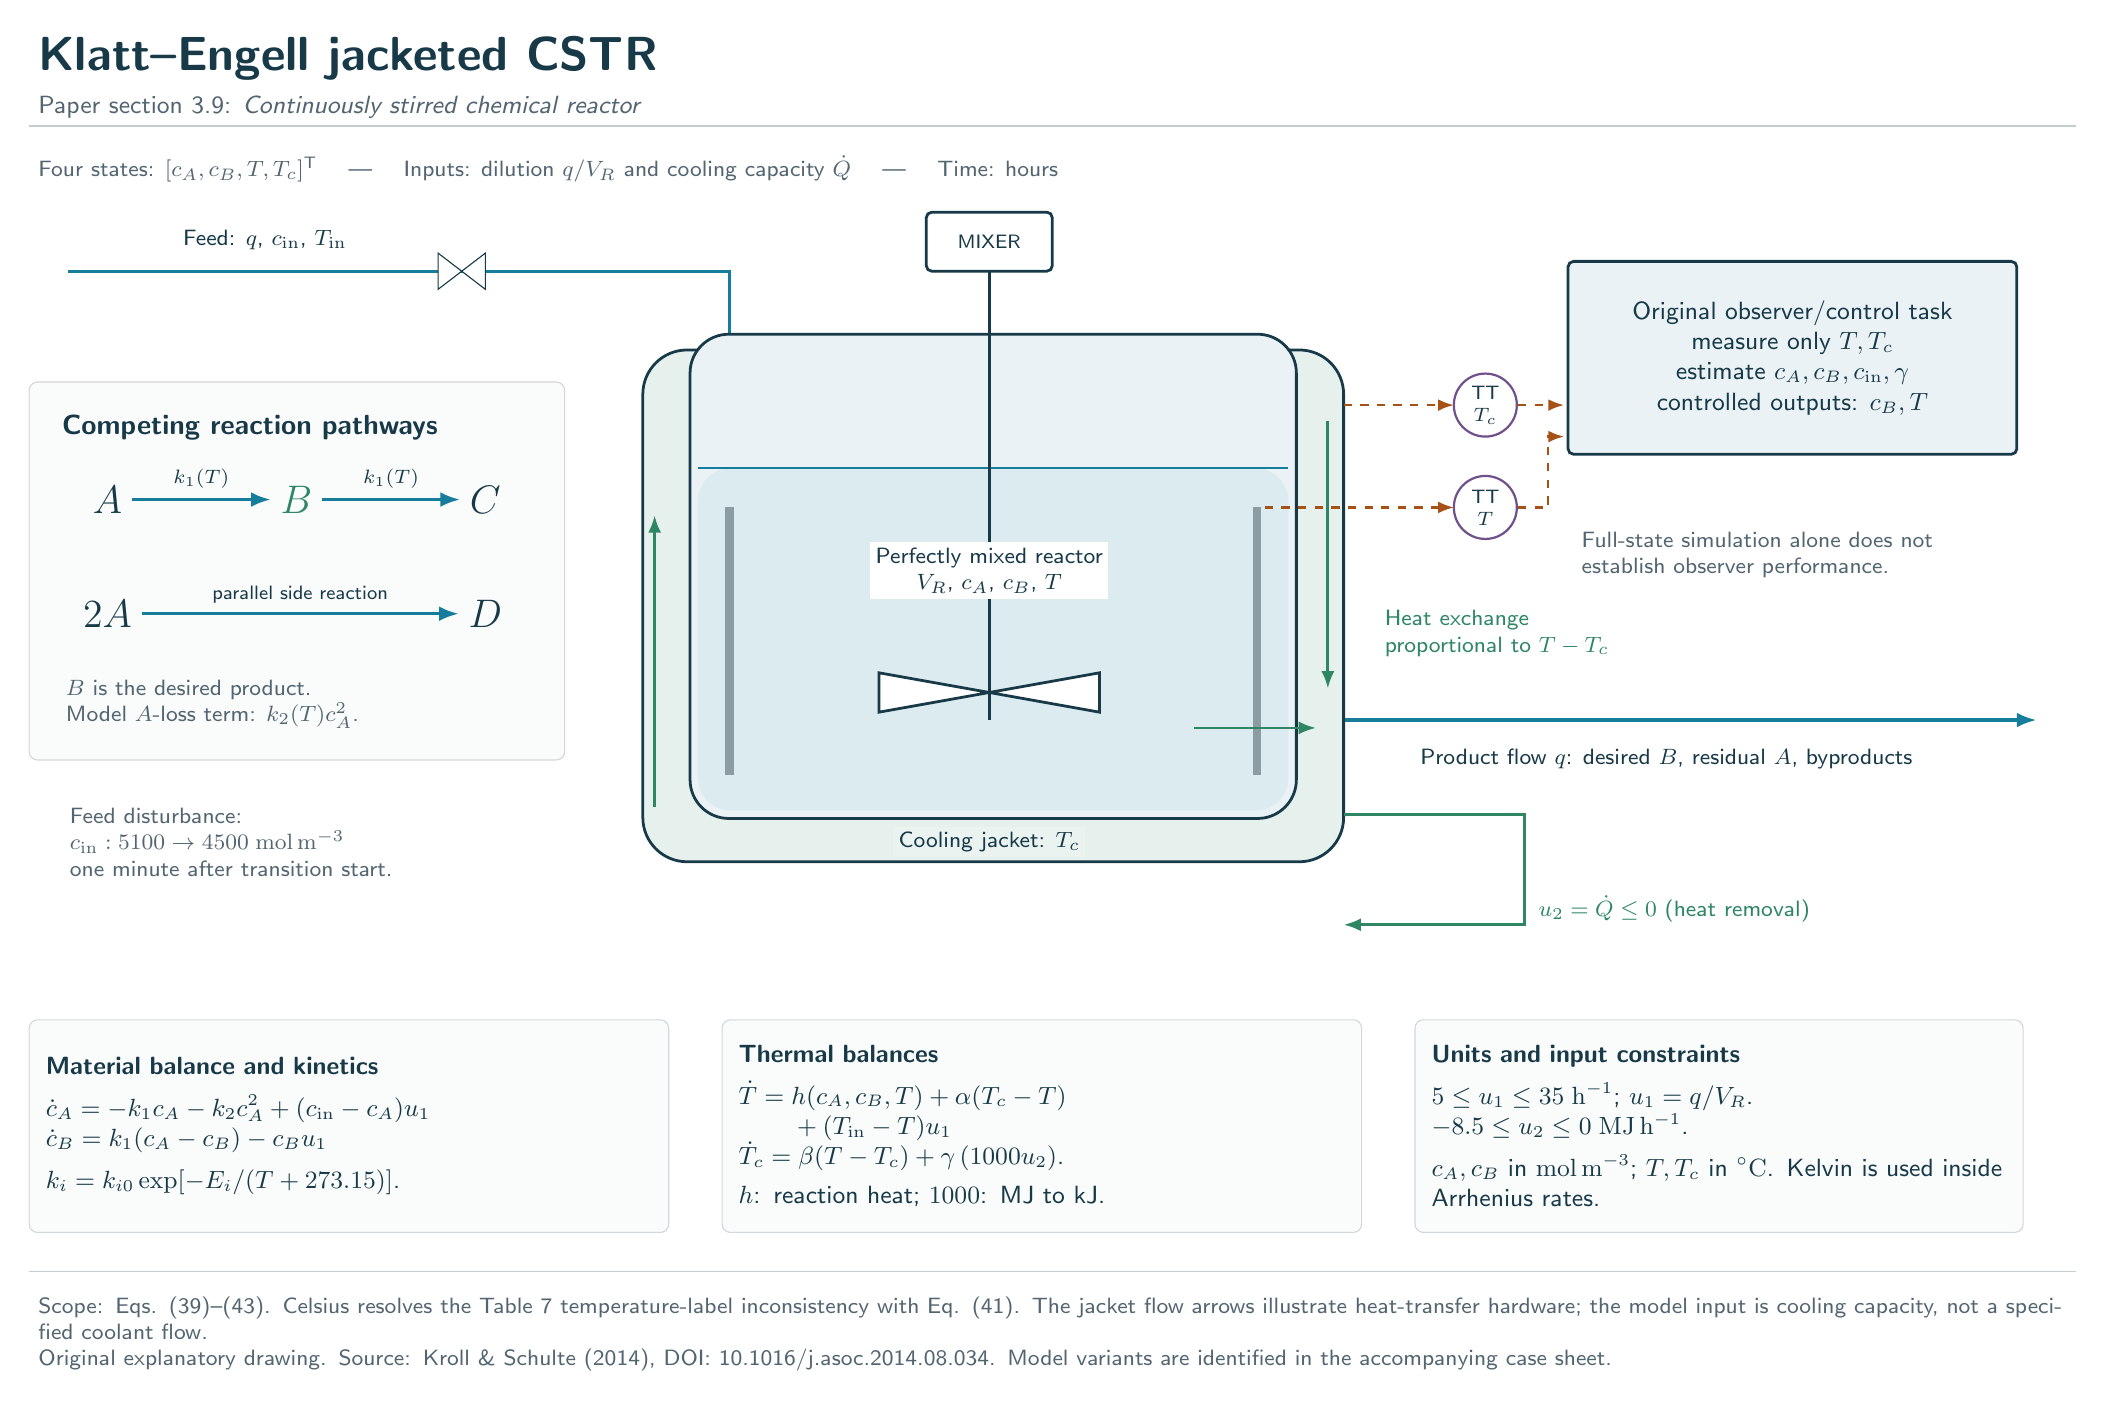
\begin{tikzpicture}[x=1cm,y=1cm]
\atlasheader{Klatt--Engell jacketed CSTR}{3.9}{Continuously stirred chemical reactor}
\node[annotation,anchor=west] at (0,-1.8) {Four states: $[c_A,c_B,T,T_c]^{\mathsf T}$ \quad | \quad Inputs: dilution $q/V_R$ and cooling capacity $\dot Q$ \quad | \quad Time: hours};
% Inlet and outlet, with a valve indicating the dilution input.
\draw[process] (.5,-3.1)--(8.9,-3.1)--(8.9,-5.3);
\draw[ink,fill=white] (5.2,-2.87)--(5.8,-3.33)--(5.8,-2.87)--(5.2,-3.33)--cycle;
\node[labelbox] at (3,-2.7) {Feed: $q$, $c_{\mathrm{in}}$, $T_{\mathrm{in}}$};
\draw[process] (16,-8.8)--(25.5,-8.8);
\node[labelbox] at (20.8,-9.3) {Product flow $q$: desired $B$, residual $A$, byproducts};
% Rounded cooling jacket encloses the reactor, with distinct coolant color.
\path[equipment,fill=utility!12,rounded corners=16pt] (7.8,-4.1) rectangle (16.7,-10.6);
\path[equipment,fill=pale,rounded corners=14pt] (8.4,-3.9) rectangle (16.1,-10.05);
\path[fill=flow!15,rounded corners=12pt] (8.5,-5.6) rectangle (16,-9.95);
\draw[flow,line width=.8pt] (8.5,-5.6)--(16,-5.6);
\draw[ink!50,line width=3pt] (8.9,-6.1)--(8.9,-9.5) (15.6,-6.1)--(15.6,-9.5);
\draw[equipment,fill=white] (11.4,-2.35) rectangle (13,-3.1);
\node[font=\sffamily\scriptsize] at (12.2,-2.73) {MIXER};
\draw[ink,line width=1.2pt] (12.2,-3.1)--(12.2,-8.8);
\draw[ink,fill=white,line width=1pt] (10.8,-8.2)--(13.6,-8.7)--(13.6,-8.2)--(10.8,-8.7)--cycle;
\node[labelbox,align=center] at (12.2,-6.9) {Perfectly mixed reactor\\$V_R$, $c_A$, $c_B$, $T$};
\node[labelbox,fill=utility!10] at (12.2,-10.35) {Cooling jacket: $T_c$};
\draw[util] (7.95,-9.9)--(7.95,-6.2);
\draw[util] (16.5,-5)--(16.5,-8.4);
\draw[util] (16.7,-10)--(19,-10)--(19,-11.4)--(16.7,-11.4);
\node[labelbox,text=utility] at (20.9,-11.2) {$u_2=\dot Q\leq0$ (heat removal)};
\draw[util] (14.8,-8.9)--(16.35,-8.9);
\node[annotation,text=utility,anchor=west] at (17.1,-7.7) {Heat exchange\\proportional to $T-T_c$};
% Reaction network separated from the process ports.
\node[panel,anchor=north west,minimum width=6.8cm,minimum height=4.8cm] at (0,-4.5) {};
\node[anchor=north west,font=\sffamily\bfseries] at (.3,-4.8) {Competing reaction pathways};
\node[font=\sffamily\Large] (a) at (1,-6) {$A$};
\node[font=\sffamily\Large,text=utility] (b) at (3.4,-6) {$B$};
\node[font=\sffamily\Large] (c) at (5.8,-6) {$C$};
\draw[process] (a)--node[above,font=\sffamily\scriptsize] {$k_1(T)$} (b);
\draw[process] (b)--node[above,font=\sffamily\scriptsize] {$k_1(T)$} (c);
\node[font=\sffamily\Large] (aa) at (1,-7.45) {$2A$};
\node[font=\sffamily\Large] (d) at (5.8,-7.45) {$D$};
\draw[process] (aa)--node[above,font=\sffamily\scriptsize] {parallel side reaction} (d);
\node[annotation,anchor=west] at (.35,-8.6) {$B$ is the desired product.\\Model $A$-loss term: $k_2(T)c_A^2$.};
\node[annotation,anchor=west] at (.4,-10.35) {Feed disturbance:\\$c_{\mathrm{in}}:5100\rightarrow4500\;\mathrm{mol\,m^{-3}}$\\one minute after transition start.};
% Temperature-only observations and original observer challenge.
\draw[signal] (15.7,-6.1)--(18.1,-6.1);
\node[instrument] (tt) at (18.5,-6.1) {TT\\$T$};
\draw[signal] (16.7,-4.8)--(18.1,-4.8);
\node[instrument] (tc) at (18.5,-4.8) {TT\\$T_c$};
\node[box,minimum width=5.7cm,minimum height=2.45cm] (obs) at (22.4,-4.2) {Original observer/control task\\measure only $T,T_c$\\estimate $c_A,c_B,c_{\mathrm{in}},\gamma$\\controlled outputs: $c_B,T$};
\draw[signal] (tc.east)--(19.5,-4.8);
\draw[signal] (tt.east)--(19.3,-6.1)--(19.3,-5.2)--(19.5,-5.2);
\node[annotation,anchor=west] at (19.6,-6.7) {Full-state simulation alone does not\\establish observer performance.};
\node[panel,anchor=north west,text width=7.7cm,minimum height=2.7cm,align=left] at (0,-12.6) {\textbf{Material balance and kinetics}\\[4pt]
 $\dot c_A=-k_1c_A-k_2c_A^2+(c_{\mathrm{in}}-c_A)u_1$\\
 $\dot c_B=k_1(c_A-c_B)-c_Bu_1$\\[4pt]
 $k_i=k_{i0}\exp[-E_i/(T+273.15)]$.};
\node[panel,anchor=north west,text width=7.7cm,minimum height=2.7cm,align=left] at (8.8,-12.6) {\textbf{Thermal balances}\\[4pt]
 $\dot T=h(c_A,c_B,T)+\alpha(T_c-T)$\\$\hphantom{\dot T={}}+(T_{\mathrm{in}}-T)u_1$\\
 $\dot T_c=\beta(T-T_c)+\gamma\,(1000u_2)$.\\[3pt]
 $h$: reaction heat; $1000$: MJ to kJ.};
\node[panel,anchor=north west,text width=7.3cm,minimum height=2.7cm,align=left] at (17.6,-12.6) {\textbf{Units and input constraints}\\[4pt]
 $5\leq u_1\leq35\;\mathrm{h^{-1}}$; $u_1=q/V_R$.\\
 $-8.5\leq u_2\leq0\;\mathrm{MJ\,h^{-1}}$.\\[4pt]
 $c_A,c_B$ in $\mathrm{mol\,m^{-3}}$; $T,T_c$ in $^{\circ}\mathrm C$. Kelvin is used inside Arrhenius rates.};
\atlasfooter{Scope: Eqs. (39)--(43). Celsius resolves the Table 7 temperature-label inconsistency with Eq. (41). The jacket flow arrows illustrate heat-transfer hardware; the model input is cooling capacity, not a specified coolant flow.}
\end{tikzpicture}
\end{document}
